%!TEX root = mainfile.tex

\subsection{Spitzer Space Telescope} % (fold)
\label{sub:spitzer_space_telescope}
(Dorothy with contributions from Catherine)

	Spitzer Space telescope was launched by NASA on 25th August 2003\cite{fast_facts_spitzer} and is designed for use in the infrared. It was the last of NASA's ``Great Observatories'', working alongside HST in the optical, Compton Gamma Ray Observatory and Chandra X-ray Observatory. The telescope is \SI{85}{\centi\metre} in diameter, and sits in an Earth-trailing orbit around the Sun, shown in Figure~\ref{fig:spitzer_orbit_LARGE}. It is a Cassegrain telescope, meaning it has primary and secondary hyperbolic mirrors to focus the light and reduce spherical aberration, in a similar manner to Hubble. The majority of Spitzer's instrumentation is now non-operational due to a lack of cryogen, but some photometry remains possible.
	\begin{figure}[htbp]
		\centering
		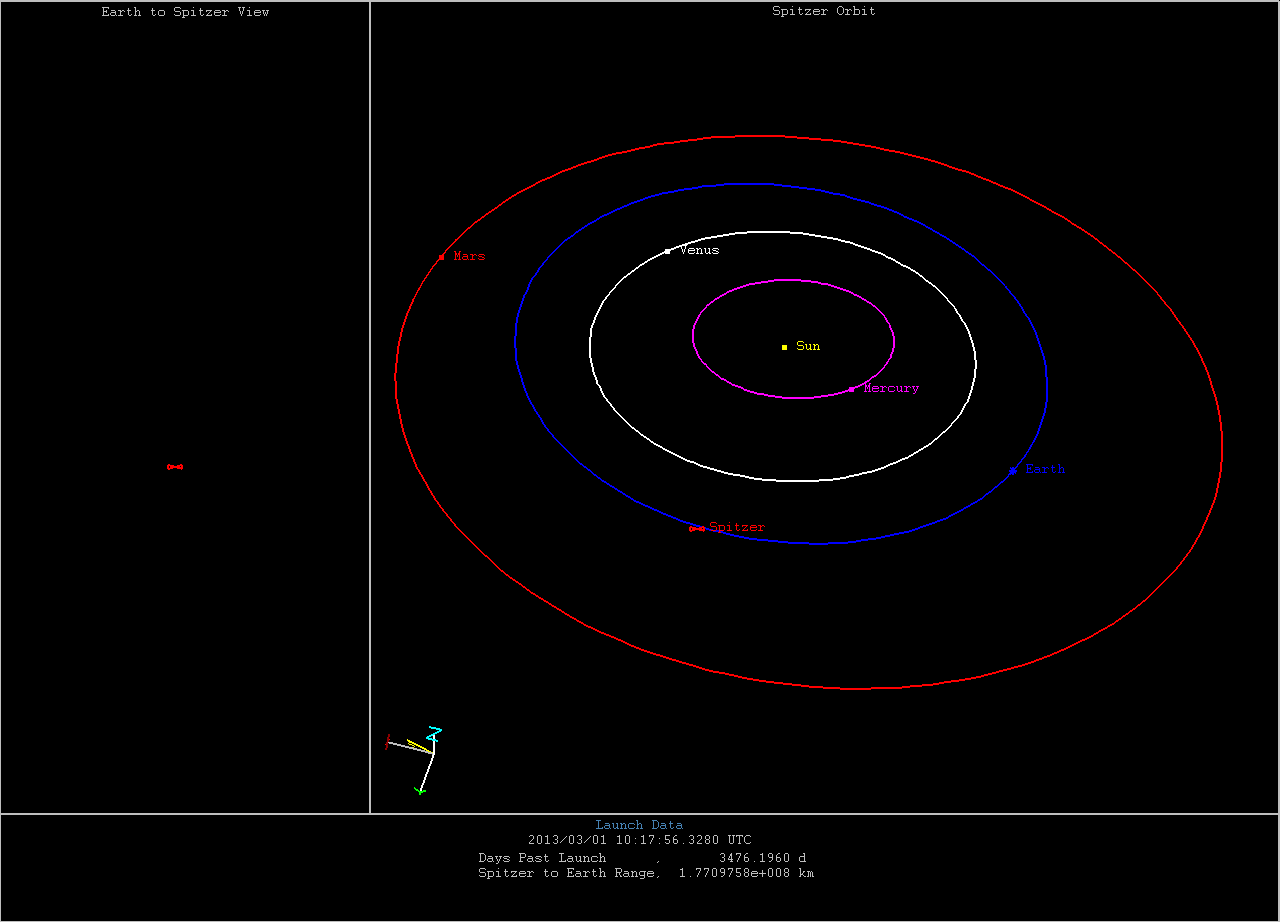
\includegraphics[trim = 110mm 70mm 5mm 30mm, clip, width=0.6\textwidth]{../Images/spitzer_orbit_LARGE.png}
		\caption{The Spitzer Space Telescope's Orbit\cite{where_is_spitzer}.\label{fig:spitzer_orbit_LARGE}}
	\end{figure}

	\subsubsection{Capabilities} % (fold)
	\label{ssub:spitzer_capabilities}
		Spitzer had the capabilities detailed in Table~\ref{tab:Spitzer_cababilities}.
		\begin{table}[htbp]
			\begin{center}
				\begin{tabular}{l|l}
					Component   &   Wavelength Range \\
					\hline\hline
					Imaging/Photometry & 3--180\si{\micro\metre} \\
					Spectroscopy       & 5--40\si{\micro\metre} \\
					Spectrophotometry  & 50--100\si{\micro\metre}
				\end{tabular}
			\end{center}
			\caption{Details of instrumentation for Spitzer\cite{WFC3_IHB}.\label{tab:Spitzer_cababilities}}
		\end{table}

		It employed three scientific instruments which helped it do the above:
		\begin{itemize}
			\item Infrared Array Camera (IRAC): an imaging camera working in the near IR at wavelengths of 3.6, 4.5, 5.8 and 8\,micrometres.
			\item Infrared Spectrograph (IRS): performing spectroscopy from 5 to 40\,micrometres.
			\item Multiband Imaging Photometer (MIPS): detected wavelengths in the far IR, at 24, 70 and 160\,micrometres.
		\end{itemize}

		The telescope was cryogenically cooled to around \SI{1.4}{\kelvin}, allowing all the instruments to function without excessive thermal interference from the telescope itself. The mission, labelled the `Cold Mission', was estimated to last between 2 and 5 years, depending on when the cryogen ran out. During this time, Spitzer imaged in all four NIR filters simultaneously, as well as doing spectroscopy, and some imaging in the far infrared. In 2009, when the cryogen ran out, the longer wavelength filters became non-operational, and the Spitzer `Warm Mission' continued imaging with the nearest IR filters ($3.6$ and $4.5$\,micrometres). This was made possible because Spitzer's orbit keeps it substantially cooler than an Earth-centred orbit would, due to the lack of IR radiation received from Earth. Furthermore it is made mostly of beryllium which has a low heat capacity at low temperatures, helping to keep it cool.

		In order to keep enough sunlight on the solar panels, Spitzer cannot point further than 120\,degrees away from the Sun. However, it also cannot get closer than 80\,degrees towards the Sun in case damage is done to the scientific instruments. This is a limitation on the area of sky which can be observed, meaning that some regions can only be seen for 40 days semi-annually, whilst other areas can be observed all year round.

		The spectrograph (IRS) operated at wavelengths too long to be of use to study the EoR, as did the far IR photometry (MIPS), however the near IR photometry capabilities of both the Spitzer warm and cold missions have been used to study high redshift galaxies, and in conjunction with HST have confirmed galaxies at redshifts as far back as $z\approx10$. Particularly the 3.6 and 4.5\,micrometre filters observe significant flux from such galaxies, and so these have been used in a number of studies looking for high redshift galaxies.
	% subsubsection capabilities (end)

    \subsubsection{Studies Involving Spitzer} % (fold)
	\label{ssub:studies_involving_spitzer}
		Coe et al (2012)\cite{0004-637X-762-1-32} reports a $z\approx11$ candidate which had been observed using HST (WFC3, ACS) and Spitzer (IRAC) for longer wavelengths. This is one of the highest redshift candidates to date. The Spitzer data was taken over a total integration time of 5 hours.

		An earlier study in 2008 by Richard et al also used Hubble to detect galaxies greater than redshift seven (making use of gravitational lenses). Spitzer imaged these galaxies to help confirm that they were not foreground objects of a different nature, by looking at the flux in longer wavelength filters\cite{0004-637X-685-2-705}.

		In 2005, during the cold mission, a study was made by Spitzer on a confirmed $z=6.56$ galaxy (HCM 6A) lensed by a cluster (Abell 370). The study was used to detect the rest frame optical emission of this galaxy in order to better understand the physical properties of objects at such high redshifts\cite{1538-4357-635-1-L5}. Several other papers have also used Spitzer data in the study of high redshift galaxies.

		Spitzer also has ideal filters to look at the Balmer or \SI{4000}{\angstrom} break which, if prominent, would indicate an older stellar population and suggest that the object is more likely a contaminant than a high redshift LBG, since high redshift LBGs do not contain many old stars.

		The data in Table~\ref{tab:Spitzer_technical} shows some of the key technical data availible for the telescope.
		\begin{table}[htbp]
			\begin{center}
				\begin{tabular}{l|l}
					Component   &   Details \\
					\hline\hline
					Primary mirror & \SI{0.85}{\metre} \\
					FoV & \SI{5.2}{\arcminute}$\times$\SI{5.2}{\arcminute} \\
					Pixel size & \SI{1.2}{\arcsecond}$\times$\SI{1.2}{\arcsecond} \\
					Detector Array & $256\times256$\,\si{\pixel} \\
					\multirow{2}{*}{Full well} & 145,000 at \SI{3.6}{\micro\metre} \\
							& 140,000 at \SI{4.5}{\micro\metre} \\
				\end{tabular}
			\end{center}
			\caption{Technical data for Spitzer\cite{Spitzer_Heritage_Archive_Documentation}.\label{tab:Spitzer_technical}}
		\end{table}
	% subsubsection studies_involving_spitzer (end)
% subsection spitzer_space_telescope (end)
